%!TEX root = ../main.tex
%
% フランク-ヘルツの実験
% レポート用紙
%

\stepcounter{section}
\section*{フランク=ヘルツの実験}

\begin{center}
\begin{tabular}{|c|c|c|c|}
\hline
\parbox[c][1.2cm][c]{0cm}{}学籍番号 & \hspace{3cm} & 名前 & \hspace{6cm} \\
\hline
\parbox[c][1.2cm][c]{0cm}{}実験日時 & \multicolumn{3}{|l|}{   年  月  日  曜日  時限}\\
\hline
\parbox[c][2.0cm][c]{0cm}{}共同実験者 & \multicolumn{3}{|l|}{}\\
\hline
\end{tabular}
\end{center}

\subsection*{実験の概要と目的}

\newpage

\subsection*{測定値および計算}

\subjikken{}

\subsubsection*{測定前機器調整チェックリスト}

\begin{tabular}{|r|p{14cm}|p{0.7cm}|}
\hline
1 & POWER: OFF & \\
\hline
2 & すべてのつまみを左いっぱいにまわす & \\
\hline
3 & 切り替えスイッチ: MANU, OSC, INTERNAL, SHORT & \\
\hline
4 & 電源コード接続、POWER: ON & \\
\hline
5 & GAIN: マークを真上 & \\
\hline
6 & ZERO.ADJ.: 電流計ゼロ調整(安定するまで2〜3分待つ) & \\
\hline
7 & G${}_2$-K.VOL.ADJ.: 電圧計30V &\\
\hline
8 & HEATER.VOL.ADJ.: マーク真上 & \\
\hline
9 & G${}_1$-K.VOL.ADJ.: 電流計の指針がよくふれる位置(指針は目盛りの中央) & \\
\hline
10 & G${}_2$-K.VOL.ADJ.: 左いっぱい戻す & \\ 
\hline
11 & ZERO.ADJ.: 電流計ゼロ調整 & \\
\hline
12 & G${}_2$-K.VOL.ADJ.: 電圧計30V &\\
\hline
13 &  G${}_2$-P.VOL.ADJ.: ゆっくりと右、電流計の指針をふれの2/3ぐらいまで下げる &\\
\hline
14 & G${}_2$-K.VOL.ADJ.: 左いっぱい戻す & \\ 
\hline
15 &  G${}_2$-K.VOL.ADJ.: ゆっくりと右、電圧計と電流計の値を記録していく(測定)  & \\
\hline
\end{tabular}

\subsubsection*{測定値}
\hspace*{-\parindent}
\begin{tabular}{|c|c||c|c||c|c||c|c|}
\hline
\scriptsize 加速電圧 & \scriptsize プレート電流 & \scriptsize 加速電圧 & \scriptsize プレート電流 & \scriptsize 加速電圧 & \scriptsize プレート電流 & \scriptsize 加速電圧 & \scriptsize プレート電流 \\
\hline\hline
\hspace*{1.6cm}&\hspace*{1.6cm}&\hspace*{1.6cm}&\hspace*{1.6cm}&\hspace*{1.6cm}&\hspace*{1.6cm}&\hspace*{1.6cm}&\hspace*{1.6cm}\\
\hline
&&&&&&&\\
\hline
&&&&&&&\\
\hline
&&&&&&&\\
\hline
&&&&&&&\\
\hline
&&&&&&&\\
\hline
&&&&&&&\\
\hline
&&&&&&&\\
\hline
&&&&&&&\\
\hline
&&&&&&&\\
\hline
&&&&&&&\\
\hline
&&&&&&&\\
\hline
&&&&&&&\\
\hline
&&&&&&&\\
\hline
&&&&&&&\\
\hline
&&&&&&&\\
\hline
&&&&&&&\\
\hline
&&&&&&&\\
\hline
&&&&&&&\\
\hline
&&&&&&&\\
\hline
&&&&&&&\\
\hline
&&&&&&&\\
\hline
&&&&&&&\\
\hline
&&&&&&&\\
\hline
&&&&&&&\\
\hline
\end{tabular}

\subsubsection*{プロット}
\bigskip\bigskip
\hspace*{-\parindent}
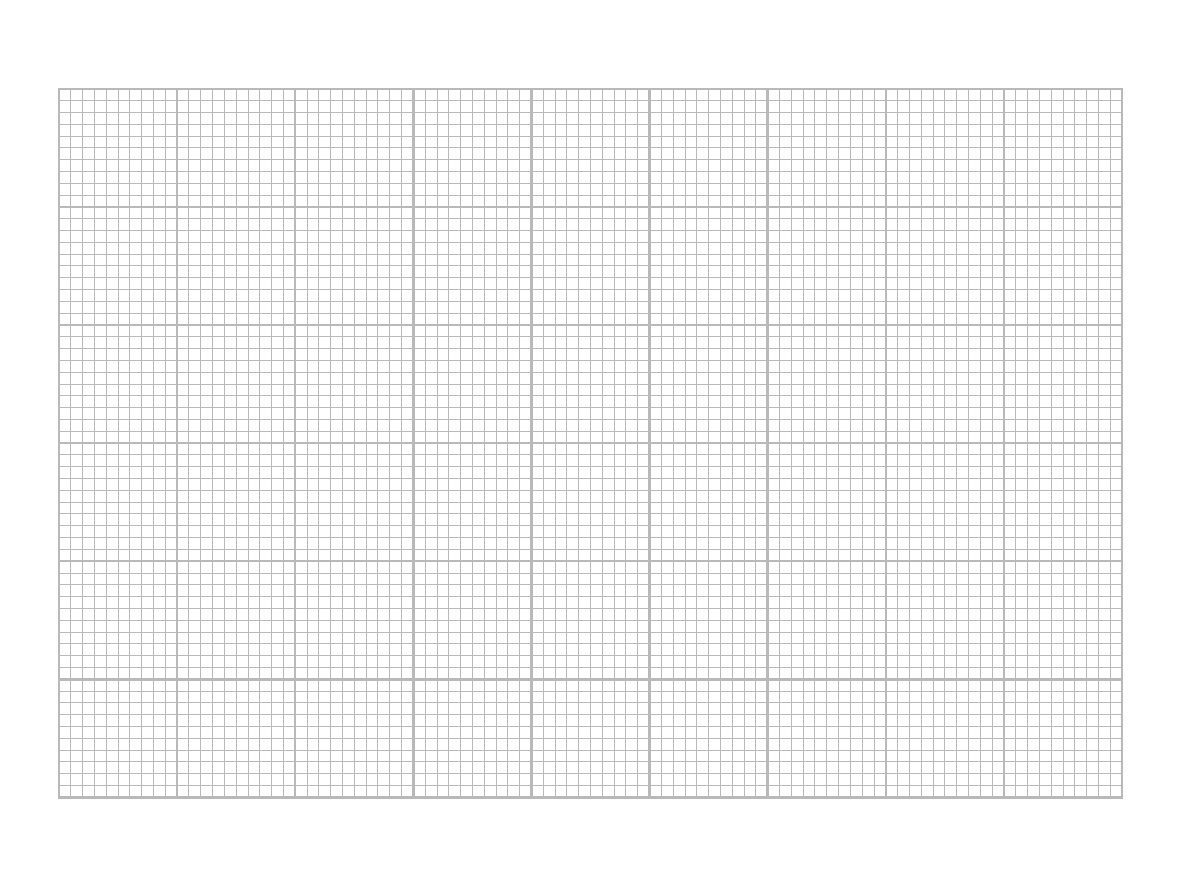
\includegraphics[scale=0.93, bb=33 32 365 362]{13_FranckHertz/graph.pdf}

\vspace*{2cm}


\subsubsection*{プレート電流ピーク時の加速電圧}

\hspace*{-\parindent}
\begin{tabular}{|r|c|}
\hline
No & 加速電圧 $V_n$ [V]\\
\hline\hline
1 & \\\hline
2 & \\\hline
3 & \\\hline
4 & \\\hline
5 & \\\hline
6 & \\\hline
\end{tabular}

\subsubsection*{各ピーク時の加速電圧の差}

\hspace*{-\parindent}
\begin{tabular}{|r|c|}
\hline
$n$ & $V_{n+1}-V_n$ [V]\\
\hline\hline
1 & $V_2-V_1=$ \hspace{5cm} \\\hline
2 & $V_3-V_2=$ \hspace{5cm} \\\hline
3 & $V_4-V_3=$ \hspace{5cm} \\\hline
4 & $V_5-V_4=$ \hspace{5cm} \\\hline
5 & $V_6-V_5=$ \hspace{5cm} \\\hline
\end{tabular}

\subsubsection*{加速電圧の差の平均}
\[
\overline{V_{n+1}-V_n}=\hspace{5cm} \text{[V]}
\]


\subsection*{考察}

\begin{itemize}

\item フランク=ヘルツ管の中にあるグリッド1(${\rm G}_1$)とグリッド2(${\rm G}_2$)のそれぞれの役割について考察してみましょう。

\vspace{5cm}

\item フランク=ヘルツの実験からどのようなことを結論づけることができるでしょうか?


\end{itemize}

